\documentclass[letterpaper,11pt]{article}

\usepackage{amsmath, amsfonts, amssymb, amsthm}
\usepackage{lmodern}
\usepackage{enumitem}
\usepackage{hyperref}
\usepackage[x11names, rgb]{xcolor}
\usepackage{graphicx}
\usepackage{fullpage}
\usepackage{etoolbox}
\usepackage{mathtools}

\setlength{\parindent}{0pt}
\setlength{\parskip}{6pt}

\newcommand{\cX}{\mathcal{X}}
\newcommand{\cC}{\mathcal{C}}
\newcommand{\cF}{\mathcal{F}}
\newcommand{\R}{\mathbb{R}}
\newcommand{\dd}{{\rm d}}
\DeclareMathOperator{\sech}{sech}

\newcommand{\nopagenumbers}{
    \pagestyle{empty}
}

\newenvironment{indented}{
    \begin{list}{}{\leftmargin=1em}
    \item[]
}{
    \end{list}
}

\newtoggle{questionnumbers}
\toggletrue{questionnumbers}

\newcounter{questionCounter}
\newcounter{partCounter}[questionCounter]

\newcommand{\question}[1]{%
    \stepcounter{questionCounter}%
    \setcounter{partCounter}{0}%
    \vspace{0.25in}
    \hrule
    \vspace{0.4em}
    \noindent\textbf{Question \thequestionCounter:\ }#1
    \vspace{0.8em}
    \hrule
    \vspace{0.1in}
}

\newcommand{\qpart}[1]{%
    \stepcounter{partCounter}%
    \begin{indented}
    \textbf{(\alph{partCounter}) }#1\par
}

\newcommand{\closepart}{
    \end{indented}
}

\newcommand{\myhwname}{AMATH 353 HW 6}
\newcommand{\myname}{Jordan Tucker}

\newcommand{\header}{
    \begin{center}
    {\Large \myhwname}\\
    \myname\\
    \today
    \end{center}
}

\nopagenumbers
\begin{document}
    \header
    \question{Method of Characteristics (part 1)}
    \qpart{Find the characteristic curves of the PDE
        \[
            u_t + xu_x=0.
        \] Sketch/plot the characteristic curves in the $xt$-plane. What do you predict the dynamics tolook like?}
    \begin{gather*}
        u_t + xu_x = 0\\
        \frac{d}{dt} u(x(t),t) = u_t + \frac{dx}{dt} u_x\\
        u_t + \frac{dx}{dt} u_x = u_t + xu_x\\
        \frac{dx}{dt} = x\\
    \end{gather*}
    Solve the ODE:
    \begin{gather*}
        \frac{1}{x} dx = dt\\
        \int \frac{1}{x} dx = \int dt\\
        \ln|x| = t + \ln|x_0|\\
        x = e^{t+ \ln|x_0|}\\
        x = x_0 e^t
    \end{gather*}
    The wave will go faster the further it gets from the origin.
    If $x_0 > 0$ it moves to the right.
    If $x_0 < 0$ it moves to the left.
    \begin{center}
        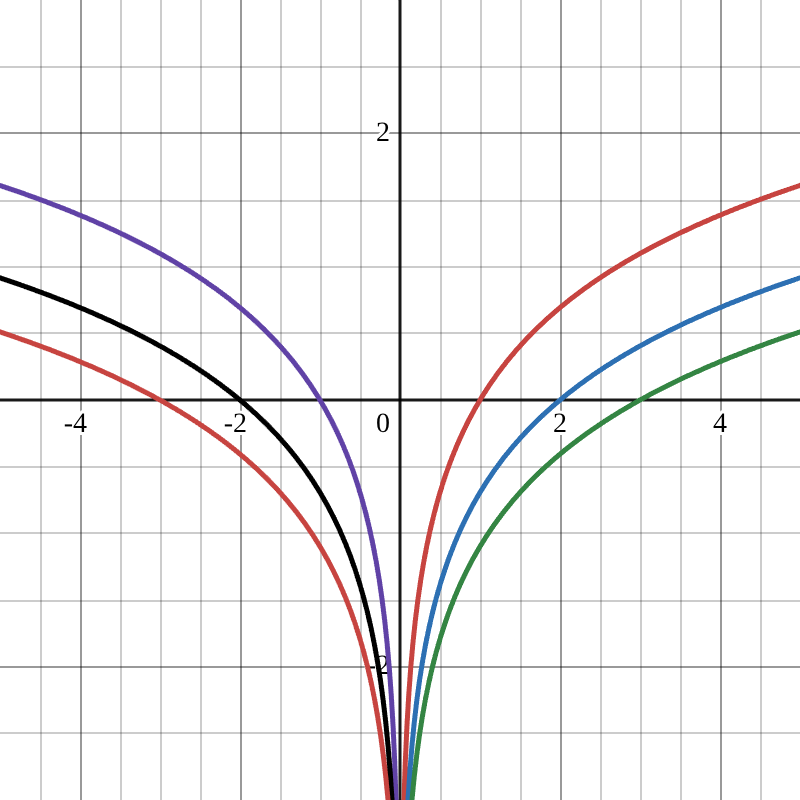
\includegraphics[width=0.5\textwidth]{hw6chart}
    \end{center}
    \closepart
    \qpart{Use the method of characteristics to solve
        \[
            \begin{cases}
                u_t + tu_x = 0, & x \in \R, t \ge 0,\\
                u(x,0) =  \cos(x), & x \in \R, t \ge 0.\\
            \end{cases}
        \] Give a qualitative description of the dynamics of the solution.}
    \begin{gather*}
        u_t + t u_x = 0\\
        \frac{d}{dt} u((x),t) = u_t + \frac{dx}{dt} u_x\\
        u_t + tu_x =u_t + \frac{dx}{dt} u_x\\
        \frac{dx}{dt} = t\\
    \end{gather*}
    Solve the ODE
    \begin{gather*}
        \frac{dx}{dt} = t\\
        dx = tdt\\
        \int dx = \int t dt\\
        x = \frac{t^2}{2} + x_0\\
        x_0 = x-\frac{t^2}{2}\\
        u(x_0, 0) = \cos(x-\frac{t^2}{2})\\\\
        u(x, t) = \cos(x-\frac{t^2}{2})
    \end{gather*}
    The wave speeds up as it moves away from $x_0$, and always moves to the right.
    \closepart
    \qpart{Use the method of characteristics to solve
        \[
            \begin{cases}
                u_t + \cos(t)u_x = 0, & x \in \R, t \ge 0,\\
                u(x,0) =  e^{-x^2}, & x \in \R, t \ge 0.\\
            \end{cases}
        \] Give a qualitative description of the dynamics of the solution.}
    \begin{gather*}
        u_t = \cos(t) u_x = 0\\
        \frac{d}{dt} u(x(t),t) = u_t + \frac{dx}{dt} u_x\\
        u_t + \frac{dx}{dt} u_x = u_t + \cos(t)u_x\\
        \frac{dx}{dt} = \cos(t)
    \end{gather*}
    Solve the ODE
    \begin{gather*}
        \frac{dx}{dt} = \cos(t)\\
        dx = \cos(t) dt\\
        \int dx = \int \cos(t) dt\\
        x = \sin(t) + x_0\\
        x_0 = x - \sin(t)\\\\
        u(x_0, 0) = e ^{-(x-\sin(t))^2}\\
        u(x,t) = e ^{-(x-\sin(t))^2}
    \end{gather*}
    The wave bounces between $-1$ and $1$, and the velocity depends on time.
    \closepart
    \newpage
    \question{Method of Characteristics (part 2)}
    \qpart{Determine the (implicit) solution to
    the nonlinear, homogeneous PDE problem
        \[
            \begin{cases}
                u_t + u^2u_x = 0,& x \in \R, t \ge 0,\\
                u(x,0) = \tanh(x), & x \in \R.\\
            \end{cases}
        \]}
    \begin{gather*}
        x = x(t)\\
        \frac{d}{dt} u(x(t),t) = u_t + \frac{dx}{dt} u_x\\
        u_t + \frac{dx}{dt} u_x = u_t = u^2 u_x\\
        \frac{dx}{dt} = u^2\\
    \end{gather*}
    Solve The ODE
    \begin{gather*}
        \frac{dx}{dt} = u^2\\
        dx = u^2 dt\\
        \int dx = \int u^2 dt\\
        x= u^2 t + x_0\\
        x_0 = x - u^2 t\\
        u(x_0, 0) = \tanh (x_0)\\
        u(x,t) = \tanh(x_0)\\
        u(x,t) = \tanh(x-u^2t)
    \end{gather*}
    \closepart
    \qpart{Determine the (explicit) solution to
    the linear, in-homogeneous PDE problem
        \[
            \begin{cases}
                u_t + 2tu_x = 2t\cos(x),& x \in \R, t \ge 0,\\
                u(x,0) = \sech^2(x), & x \in \R.\\
            \end{cases}
        \]}
    \begin{gather*}
        \frac{d}{dt} u(x(t),t) = u_t + \frac{dx}{dt} u_x\\
        u_t + \frac{dx}{dt} u_x = u_t + 2tu_x\\
        \frac{dx}{dt} = 2t
    \end{gather*}
    Solve the ODE
    \begin{gather*}
        \frac{dx}{dt} = 2t\\
        dx = 2t dt\\
        \int dx =\int 2t dt\\
        x = t^2 + x_0\\\\
        \frac{du}{dt} = 2t \cos(x(t))\\
        \int du = \int 2t \cos(t^2 +x_0) dt\\
        u(t) = \sin(t^2 + x_0) + C
    \end{gather*}
    Initial Conditions
    \begin{gather*}
        t = 0, \ u(x,0) = \sech^2(x)\\
        t = 0, \ x(0) = x_0\\
        t = 0, \ u(0) = \sin(x_0) + C \\
        \sin(x_0) + C = \sech^2(x_0) \\
        C = \sech^2(x_0) - \sin(x_0)\\\\
        u(x_0,t) = \sin(t^2 + x_0) + \sech^2(x_0) - \sin(x_0)\\\\
        x = t^2 + x_0\\
        x_0 = x - t^2\\
        u(x,t) = \sin(t^2 +(x-t^2)) + \sech^2(x-t^2) - \sin(x-t^2)
    \end{gather*}
    \closepart

    \qpart{Determine the (explicit) solution to
    the non-linear, in-homogeneous PDE problem
        \[
            \begin{cases}
                u_t + uu_x = \cos(t),& x \in \R, t \ge 0,\\
                u(x,0) = x, & x \in \R.\\
            \end{cases}
        \]}
    \begin{gather*}
        \frac{d}{dt} u(x(t),t) = u_t + \frac{dx}{dt} u_x\\
        u_t + \frac{dx}{dt} u_x = u_t + uu_x\\
        \frac{dx}{dt} = u
    \end{gather*}
    Solve for $u$
    \begin{gather*}
        \frac{du}{dt} = \cos(t)\\
        \int du = \int \cos(t) dt\\
        u(t) = \sin(t) + C
    \end{gather*}
    Initial Conditions:
    \begin{gather*}
        t = 0, \ u(0) = \sin(0) + C = C\\
        C = x_0\\
        u(t) = \sin(t) + x_0
    \end{gather*}
    Solve for $x$
    \begin{gather*}
        \frac{dx}{dt} = u = \sin(t) + x_0\\
        \int dx = \int (\sin(t) + x_0) dt\\
        x(t) = -\cos(t) + x_0t + C_2\\
        t = 0, \ x(0) = -\cos(0) + x_0(0) + C_2 = -1 + C_2 = x_0\\
        C_2 = x_0 + 1\\
        x(t) = -\cos(t) + x_0t + x_0 + 1\\
        x_0(t+1) = x + \cos(t) - 1\\
        x_0 = \frac{x+\cos(t)-1}{t+1}\\
        u(x,t) = \sin(t) + \frac{x+\cos(t)-1}{t+1}
    \end{gather*}
    \closepart
    \newpage
    \question{Breaking Time}
    The breaking time $t_b$ is the first (non-negative) time at which characteristics intersect, and we computed
    \[
        t_b = \min_{x_0 \in \R}\bigg\{\frac{-1}{c'(u_0(x_0))u_0'(x_0)} \ge 0\bigg\}
        \quad \text{for} \quad
        \begin{cases}
            u_t + c(u)u_x = 0, & x\in \R, t \ge 0,\\
            u(x,0) = u_0(x), & x\in \R.\\
        \end{cases}
    \]
    For each of the following problems, determine whether the solutions breaks and if so, compute the breaking point $(x_b,t_b)$.

    \qpart{The non-viscous traffic model $u_t + v_1(1-\frac{u}{u_1})u_x = 0$
        with initial profile
        $u_0(x)= \frac{u_1}{2}e^{-(x/\beta)^2}.$
        How does $\beta$  impact the initial profile and the breaking time?}
    \begin{gather*}
        c(u) = v_1\left(1-\frac{u}{u_1}\right)\\
        c'(u) = -\frac{v_1}{u_1}\\
        u_0'(x_0) = \frac{u_1}{2}e^{-(x_0/\beta)^2}\left(\frac{-2x_0}{\beta^2}\right) = -u_1\frac{x_0}{\beta^2}e^{-(x_0/\beta)^2}\\
        t_b = \frac{-1}{\left(-\frac{v_1}{u_1}\right)\left(-u_1\frac{x_0}{\beta^2}e^{-(x_0/\beta)^2}\right)}
    \end{gather*}
    We take the derivative of the denominator with respect to $x_0$ and set it to 0 to find the minimum time
    \begin{gather*}
        \frac{d}{dx_0} \left( -\frac{v_1}{\beta^2} x_0 e^{-(x_0/\beta)^2} \right) = \frac{v_1}{\beta^2}e^{-(x_0/\beta)^2}\left[1 - \frac{2x_0^2}{\beta^2}\right] = 0\\
        1 - \frac{2x_0^2}{\beta^2} = 0 \implies x_0 = \pm\frac{\beta}{\sqrt{2}}
    \end{gather*}
    Using $x_0 = -\frac{\beta}{\sqrt{2}}$ to make the denominator positive (and $t_b$ positive):
    \begin{gather*}
        t_b = \frac{-1}{-\frac{v_1}{\beta^2}\left(\frac{\beta}{\sqrt{2}}\right)e^{-1/2}} = \frac{\beta\sqrt{2e}}{v_1}\\
        x(t) = c(u_0)t + x_0\\
        u_0\left(-\frac{\beta}{\sqrt{2}}\right) = \frac{u_1}{2}e^{-1/2} = \frac{u_1}{2\sqrt{e}}\\
        c(u_0) = v_1\left(1-\frac{1}{2\sqrt{e}}\right)\\
        x_b = v_1\left(1-\frac{1}{2\sqrt{e}}\right)\left(\frac{\beta\sqrt{2e}}{v_1}\right) - \frac{\beta}{\sqrt{2}}\\
        x_b = \beta\sqrt{2e} - \frac{\beta\sqrt{2}}{2} - \frac{\beta\sqrt{2}}{2} = \beta\sqrt{2}(\sqrt{e}-1)
    \end{gather*}
    If $\beta$ is small, the change is steep, so the cars that end up stopping move fast. If $\beta$ is large, the cars stop more gradually.
    \closepart
    \qpart{The wacky PDE $~~u_t + \sinh\Big(\sqrt{1+\exp(u)}\Big)u_x = 0$
        with initial profile
        $u_0(x)= \tanh(x).$}
    \begin{gather*}
        c(u) = \sinh\left(\sqrt{1+\exp(u)}\right)\\
        c'(u) = \cosh\left(\sqrt{1+\exp(u)}\right)\frac{e^u}{2\sqrt{1+e^u}}\\
        u_0(x_0) = \tanh(x_0)\\
        u_0'(x_0) = \sech^2(x_0)
    \end{gather*}
    The solution breaks when $t_b = \frac{-1}{c'(u_0(x_0))u_0'(x_0)} > 0$.
    Because $c'(u)$ is always positive and $u_0'(x_0) = \sech^2(x_0)$ is always positive, the product $c'(u_0(x_0))u_0'(x_0)$ is always positive.
    Therefore, $t_b$ would be negative, meaning the solution does not break for $t \ge 0$.
    \closepart
    \qpart{Find a PDE $u_t + c(x,t)u_x = 0$ and initial profile $u_0(x)$
        so that the solution becomes arbitrarily steep as $t \rightarrow +\infty$
        but never breaks.}
    We want our characteristic curves to get close but never break. Let $c(x,t) = -x$.
    \begin{gather*}
        u_t - x u_x = 0
    \end{gather*}
    Let $u_0(x) = \cos(x)$.
    \begin{gather*}
        \frac{dx}{dt} = -x \implies \int \frac{1}{x} dx = \int -1 dt\\
        \ln|x| = -t + C \implies x(t) = x_0 e^{-t}\\
        x_0 = x e^t\\
        u(x,t) = u_0(x_0) = \cos(x e^t)\\
        u_x(x,t) = -\sin(x e^t)e^t
    \end{gather*}
    As $t \to \infty$, $e^t \to \infty$, making the slope $u_x$ steep, but it never breaks.
    \closepart
    \newpage
    \question{Understanding Qualitative Behavior}
    In this problem, you will (rigorously) establish several results concerning
    the qualitative behavior of solutions to large classes of conservation laws.
    Consider the PDE problem given by
    \[
        \begin{cases}
            u_t + c(x,t,u)u_x = 0, & x\in \R, t \ge 0,\\
            u(x,0) = u_0(x), & x\in \R.\\
        \end{cases}
    \]
    \textbf{You may assume that $c(x,t,u)$ and $u_0(x)$ are smooth functions, i.e., you can
    safely differentiate them.}
    \qpart{Prove that if $c=c(t)$, then the profile never deforms, i.e., $u(x,t)$ is
    a shift of the initial condition.}
    Assume $c = c(t)$. The PDE is $u_t + c(t)u_x = 0$ with $u(x,0) = u_0(x)$.
    Solve using the method of characteristics:
    \begin{gather*}
        \frac{dx}{dt} = c(t)\\
        dx = c(t) dt \implies x = \int c(t) dt + x_0\\
        x_0 = x - \int c(t) dt\\
        u(x,t) = u(x_0, 0) = u_0(x_0) = u_0\left(x - \int c(t) dt\right)
    \end{gather*}
    This shows that $u(x,t)$ is just a shift of the original initial condition $u_0(x)$ by $\int c(t) dt$. The profile never deforms.
    \closepart
    \qpart{Prove that if $c=c(x)>0$, then the solution never breaks, regardless of $u_0(x)$.}
    Assume $c = c(x) > 0$. The characteristics are given by:
    \begin{gather*}
        \frac{dx}{dt} = c(x)\\
        \frac{du}{dt} = 0 \implies u(x,t) = u_0(x_0)
    \end{gather*}
    Since $c(x)$ is a smooth function, we can use the etxistence and uniqueness theorem for ODEs. The theorem says that for any point $(x,t)$, there is exactly one solution curve passing through it. Therefore, characteristic curves starting at different points $x_1$ and $x_2$ can never intersect, meaning the solution never breaks.
    \closepart
    \qpart{Prove that if $c=c(u) \ne \text{const.}$, then
    there exists an initial profile $u_0(x)$ corresponding to a solution
    which breaks in finite time.}
    Assume $c = c(u)$ is not constant. By the method of characteristics:
    \begin{gather*}
        x(t) = c(u_0(x_0))t + x_0\\
        u(x,t) = u_0(x_0)
    \end{gather*}
    Taking the partial derivative with respect to $x$:
    \begin{gather*}
        u_x = u_0'(x_0) \frac{\partial x_0}{\partial x}\\
        1 = c'(u_0(x_0))u_0'(x_0) \frac{\partial x_0}{\partial x} t + \frac{\partial x_0}{\partial x}\\
        \frac{\partial x_0}{\partial x} = \frac{1}{1 + c'(u_0(x_0))u_0'(x_0) t}
    \end{gather*}
    The solution breaks when the denominator is zero. Thus, we need $c'(u_0(x_0))u_0'(x_0) < 0$.
    Because $c$ is smooth and non-constant, there must be some $u$ where $c'(u) \neq 0$.
    If $c'(u) > 0$, we can choose an initial condition $u_0(x)$ with a negative slope at that point.
    If $c'(u) < 0$, we can choose an initial condition $u_0(x)$ with a positive slope at that point.
    In either case, we can make the product $c'(u_0(x_0))u_0'(x_0)$ negative, guaranteeing that the solution will break.
    \closepart
    \qpart{Prove that if $c=c(u)$ and $u_0(x)$ are both increasing functions,
        then the solution will never break.}
    Assume $c = c(u)$ and $u_0(x)$ are both increasing functions.
    This implies that $c'(u) > 0$ and $u_0'(x) > 0$ for all valid inputs.
    The breaking time is given by:
    \begin{gather*}
        t_b = \frac{-1}{c'(u_0(x_0))u_0'(x_0)}
    \end{gather*}
    Since both $c'$ and $u_0'$ are positive, their product $c'(u_0(x_0))u_0'(x_0)$ is also positive.
    Therefore $t_b$ will be negative. Thus, the solution will never break.
    \closepart
\end{document}